\documentclass{article}

\usepackage{graphicx}
\usepackage{rotating}
\usepackage{amsmath}
\usepackage{amssymb}
\usepackage{fancyhdr}
\usepackage{listings}
\usepackage{lscape}
\usepackage{multirow}
\usepackage{color}
\usepackage{amsfonts}
\usepackage{textcomp}
\usepackage{float}
\usepackage{longtable}
\usepackage{booktabs}
\usepackage[sorting=none]{biblatex}
\usepackage[margin=1in]{geometry}
\usepackage[font={small,it}]{caption}
\usepackage[table,xcdraw]{xcolor}
\usepackage{placeins}
\usepackage{breqn}
\usepackage{xepersian}





%\DeclareMathOperator*{\btie}{\bowtie}
\addbibresource{bibliography.bib}
\settextfont[Scale=1.2]{B-NAZANIN.TTF}
\setlatintextfont[Scale=1]{Times New Roman}
\renewcommand{\baselinestretch}{1.5}
\pagestyle{fancy}
\fancyhf{}
\rhead{تکلیف دوم درس آزمون نرم افزار}
\lhead{\thepage}
\rfoot{علیرضا ابره فروش}
\lfoot{9816603}
\renewcommand{\headrulewidth}{1pt}
\renewcommand{\footrulewidth}{1pt}
%%%%%%%%%%
\lstset
{
    language=[latex]tex,
    basicstyle=\ttfamily,
    commentstyle=\color{black},
    columns=fullflexible,
    keepspaces=true,
    upquote=true,
    showstringspaces=false,
    morestring=[s]\\\%,
    stringstyle=\color{black},
}
%%%%%%%%%%
%beginMatlab
\definecolor{mygreen}{RGB}{28,172,0} % color values Red, Green, Blue
\definecolor{mylilas}{RGB}{170,55,241}
%endMatlab
\begin{document}
%beginMatlab
\lstset{language=Matlab,%
    %basicstyle=\color{red},
    breaklines=true,%
    morekeywords={matlab2tikz},
    keywordstyle=\color{blue},%
    morekeywords=[2]{1}, keywordstyle=[2]{\color{black}},
    identifierstyle=\color{black},%
    stringstyle=\color{mylilas},
    commentstyle=\color{mygreen},%
    showstringspaces=false,%without this there will be a symbol in the places where there is a space
    numbers=left,%
    numberstyle={\tiny \color{black}},% size of the numbers
    numbersep=9pt, % this defines how far the numbers are from the text
    emph=[1]{for,end,break},emphstyle=[1]\color{red}, %some words to emphasise
    %emph=[2]{word1,word2}, emphstyle=[2]{style},    
}
%endMatlab
\begin{titlepage}
\begin{center}

\includegraphics[width=0.4\textwidth]{figures/IUT Logo.png}\\
        
\LARGE
\textbf{دانشگاه صنعتی اصفهان}\\
\textbf{دانشکده مهندسی برق و کامپیوتر}\\
        
\vfill
        
\huge
\textbf{عنوان: تکلیف چهارم درس ریزپردازنده}\\
        
\vfill
        
\LARGE
\textbf{نام و نام خانوادگی: علیرضا ابره فروش}\\
\textbf{شماره دانشجویی: 9816603}\\
\textbf{نیم\,سال تحصیلی: پاییز 1400}\\
\textbf{مدرّس: دکتر عارف کریمی افشار}\\
\end{center}
\end{titlepage}


%\tableofcontents
\newpage

\section{}%1
\subsection{سوال 6 فصل هفتم صفحه‌ی 178}
\subsubsection{\lr{a}}
\begin{itemize}
\item \textbf{\lr{Node coverage}: }
\begin{latin}
$
(1), (2), (3), (4), (5), (6), (7), (8), (9), (10)
$
\end{latin}

\item \textbf{\lr{Edge coverage}: }
\begin{latin}
$
(1, 4), (1, 5), (2, 5), (6, 2), (3, 6), (3, 7), (4, 8), (5, 8), (5, 9), (9, 6), (6, 10), (7, 10)
$
\end{latin}

\item \textbf{\lr{Prime path coverage}: }
\begin{latin}
\resizebox{.99\hsize}{!}
{$
(1,4,8), (1,5,8), (3,6,10), (3,7,10), (1,5,9,6,2), (1,5,9,6,10), (2,5,9,6,10),
(2,5,9,6,2), (3,6,2,5,8), (3,6,2,5,9), (5,9,6,2,5), (6,2,5,9,6), (9,6,2,5,8), (9,6,2,5,9)
$}
\end{latin}

\end{itemize}


\subsubsection{\lr{b}}
\begin{latin}
$
(1, 4, 8), (2, 5, 9), (3, 6, 10), (3, 7, 10)
$
\end{latin}

\subsubsection{\lr{c}}
\begin{latin}
$
(1,4,8), (3,6,10), (3,7,10), (1,5,9,6,2,5,8)
$
\end{latin}


\subsection{سوال 7 فصل هفتم صفحه‌ی 179}
\subsubsection{\lr{a}}
\lr{p2} و \lr{p3} مسیر تست هستند. اما از آنجایی که \lr{p1} به نود پایانی ختم نشده است نمی‌تواند مسیر تست باشد. همچنین \lr{p4} نیز مسیر تست نیست چون با نود شروع آغاز نشده است. و در نهایت \lr{p5} نیز مسیر تست نیست چون یال $(3, 2)$ وجود ندارد.
\subsubsection{\lr{b}}
\begin{itemize}
\item \textbf{\lr{Edge-pair coverage}: }
\begin{latin}
$
(1, 2, 1), (1, 2, 3), (1, 3, 1), (2, 1, 2), (2, 1, 3), (2, 3, 1), (3, 1, 2), (3, 1, 3)
$
\end{latin}
\end{itemize}

\subsubsection{\lr{c}}
هیچ یک از مسیر‌های \lr{p2} و \lr{p3} از جفت یال‌های $(3, 1, 3)$ و $(2, 1, 2)$ عبور نمی‌کند. سایر موارد کاندید هم مسیر تست نیستند.
\subsubsection{\lr{d}}
\lr{p3} مستقیما از این \lr{prime path} عبور نمی‌کند. اما \lr{p3} از \lr{prime path}ِ با \lr{sidetrip}ِ $(1, 2, 1)$ عبور می‌کند.

\section{سوال اول صفحه‌ی 187}
\subsection{\lr{a}}
\begin{figure}[H]
    \centering
    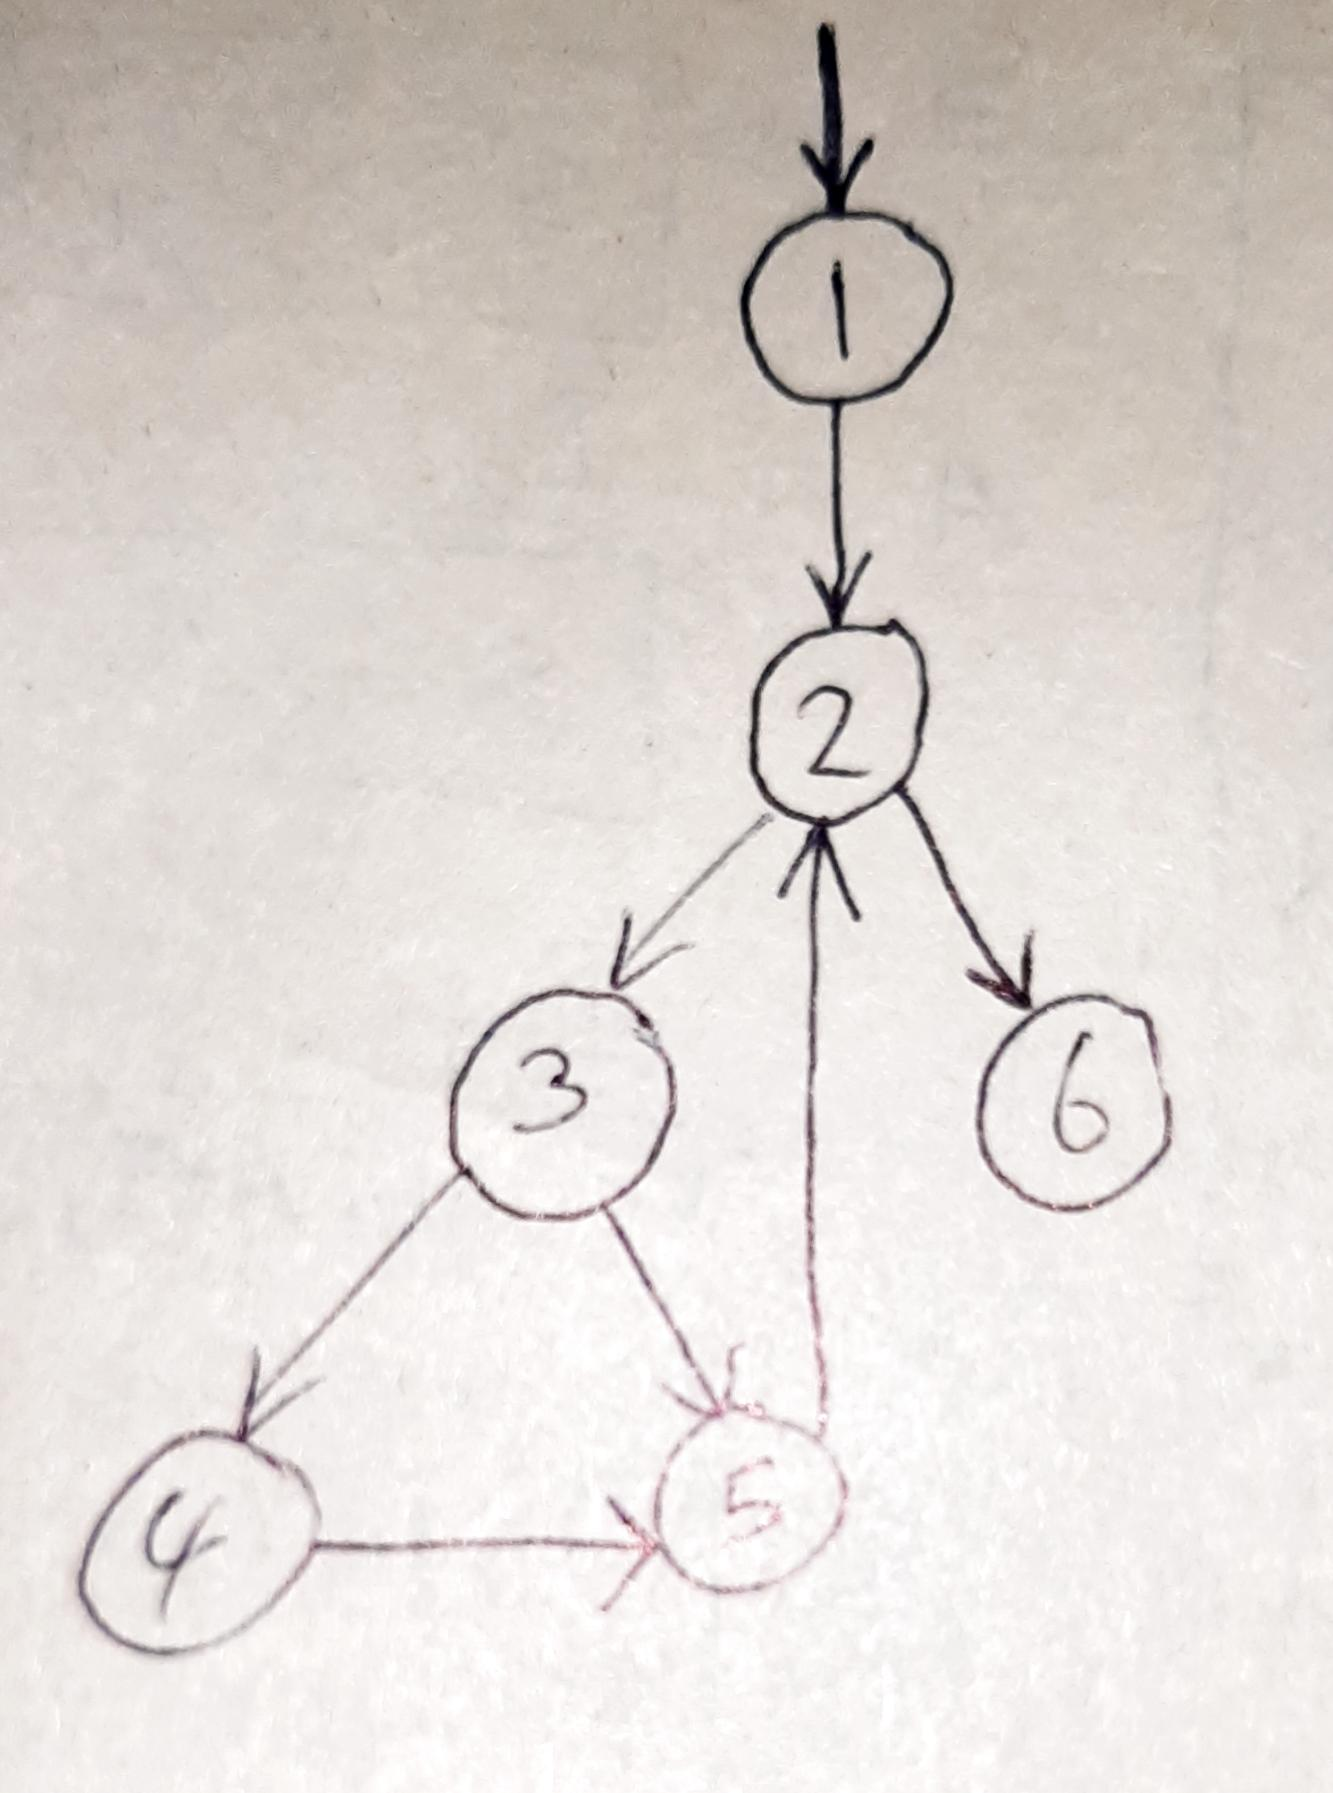
\includegraphics[width=0.25\textwidth]{figures/swt1.jpg}
    \caption
	{}
    \label{fig:fig1}
\end{figure}

\subsection{\lr{b}}
\begin{latin}
$
(1,2,6), (3,5,2,6), (1,2,3), (3,4,5,2,3), (3,5,2,3), (3,4,5,2,6)
$
\end{latin}

\subsection{\lr{c}}
\begin{latin}
\begin{table}[H]
\begin{tabular}{|c|c|}
\hline
t1: & $(1, 2, 6)$                                \\ \hline
t2: & $(3, 5, 2, 6), (3, 4, 5, 2, 3), (1, 2, 3)$ \\ \hline
t3: & $(3, 5, 2, 3), (3, 4, 5, 2, 6), (1, 2, 3)$ \\ \hline
t4: & $(3, 5, 2, 6), (1, 2, 3)$                  \\ \hline
\end{tabular}
\end{table}
\end{latin}

\subsection{\lr{d}}
\lr{def(1)} توسط همه‌ی مسیرهای تست به کار برده می‌شود و \lr{def(3)} توسط مسیرهای $\left\{ t2\right\}$ و $\left\{ t3\right\}$ و $\left\{ t4\right\}$ به کار برده می‌شود پس هر یک از مجموعه‌های $\left\{ t2\right\}$ و $\left\{ t3\right\}$ و $\left\{ t4\right\}$ می‌تواند یک مجموعه‌ی مینیمال باشد که همه‌ی \lr{def}ها را پوشش می‌دهد.

\subsection{\lr{e}}
$\left\{ t1, t2 \right\}$ و $\left\{ t1, t3 \right\}$ 

\subsection{\lr{f}}
$\left\{ t1, t2, t3 \right\}$ 


\section{سوال اول صفحات 202 و 203}
\subsection{\lr{a}}
\begin{figure}[H]
    \centering
    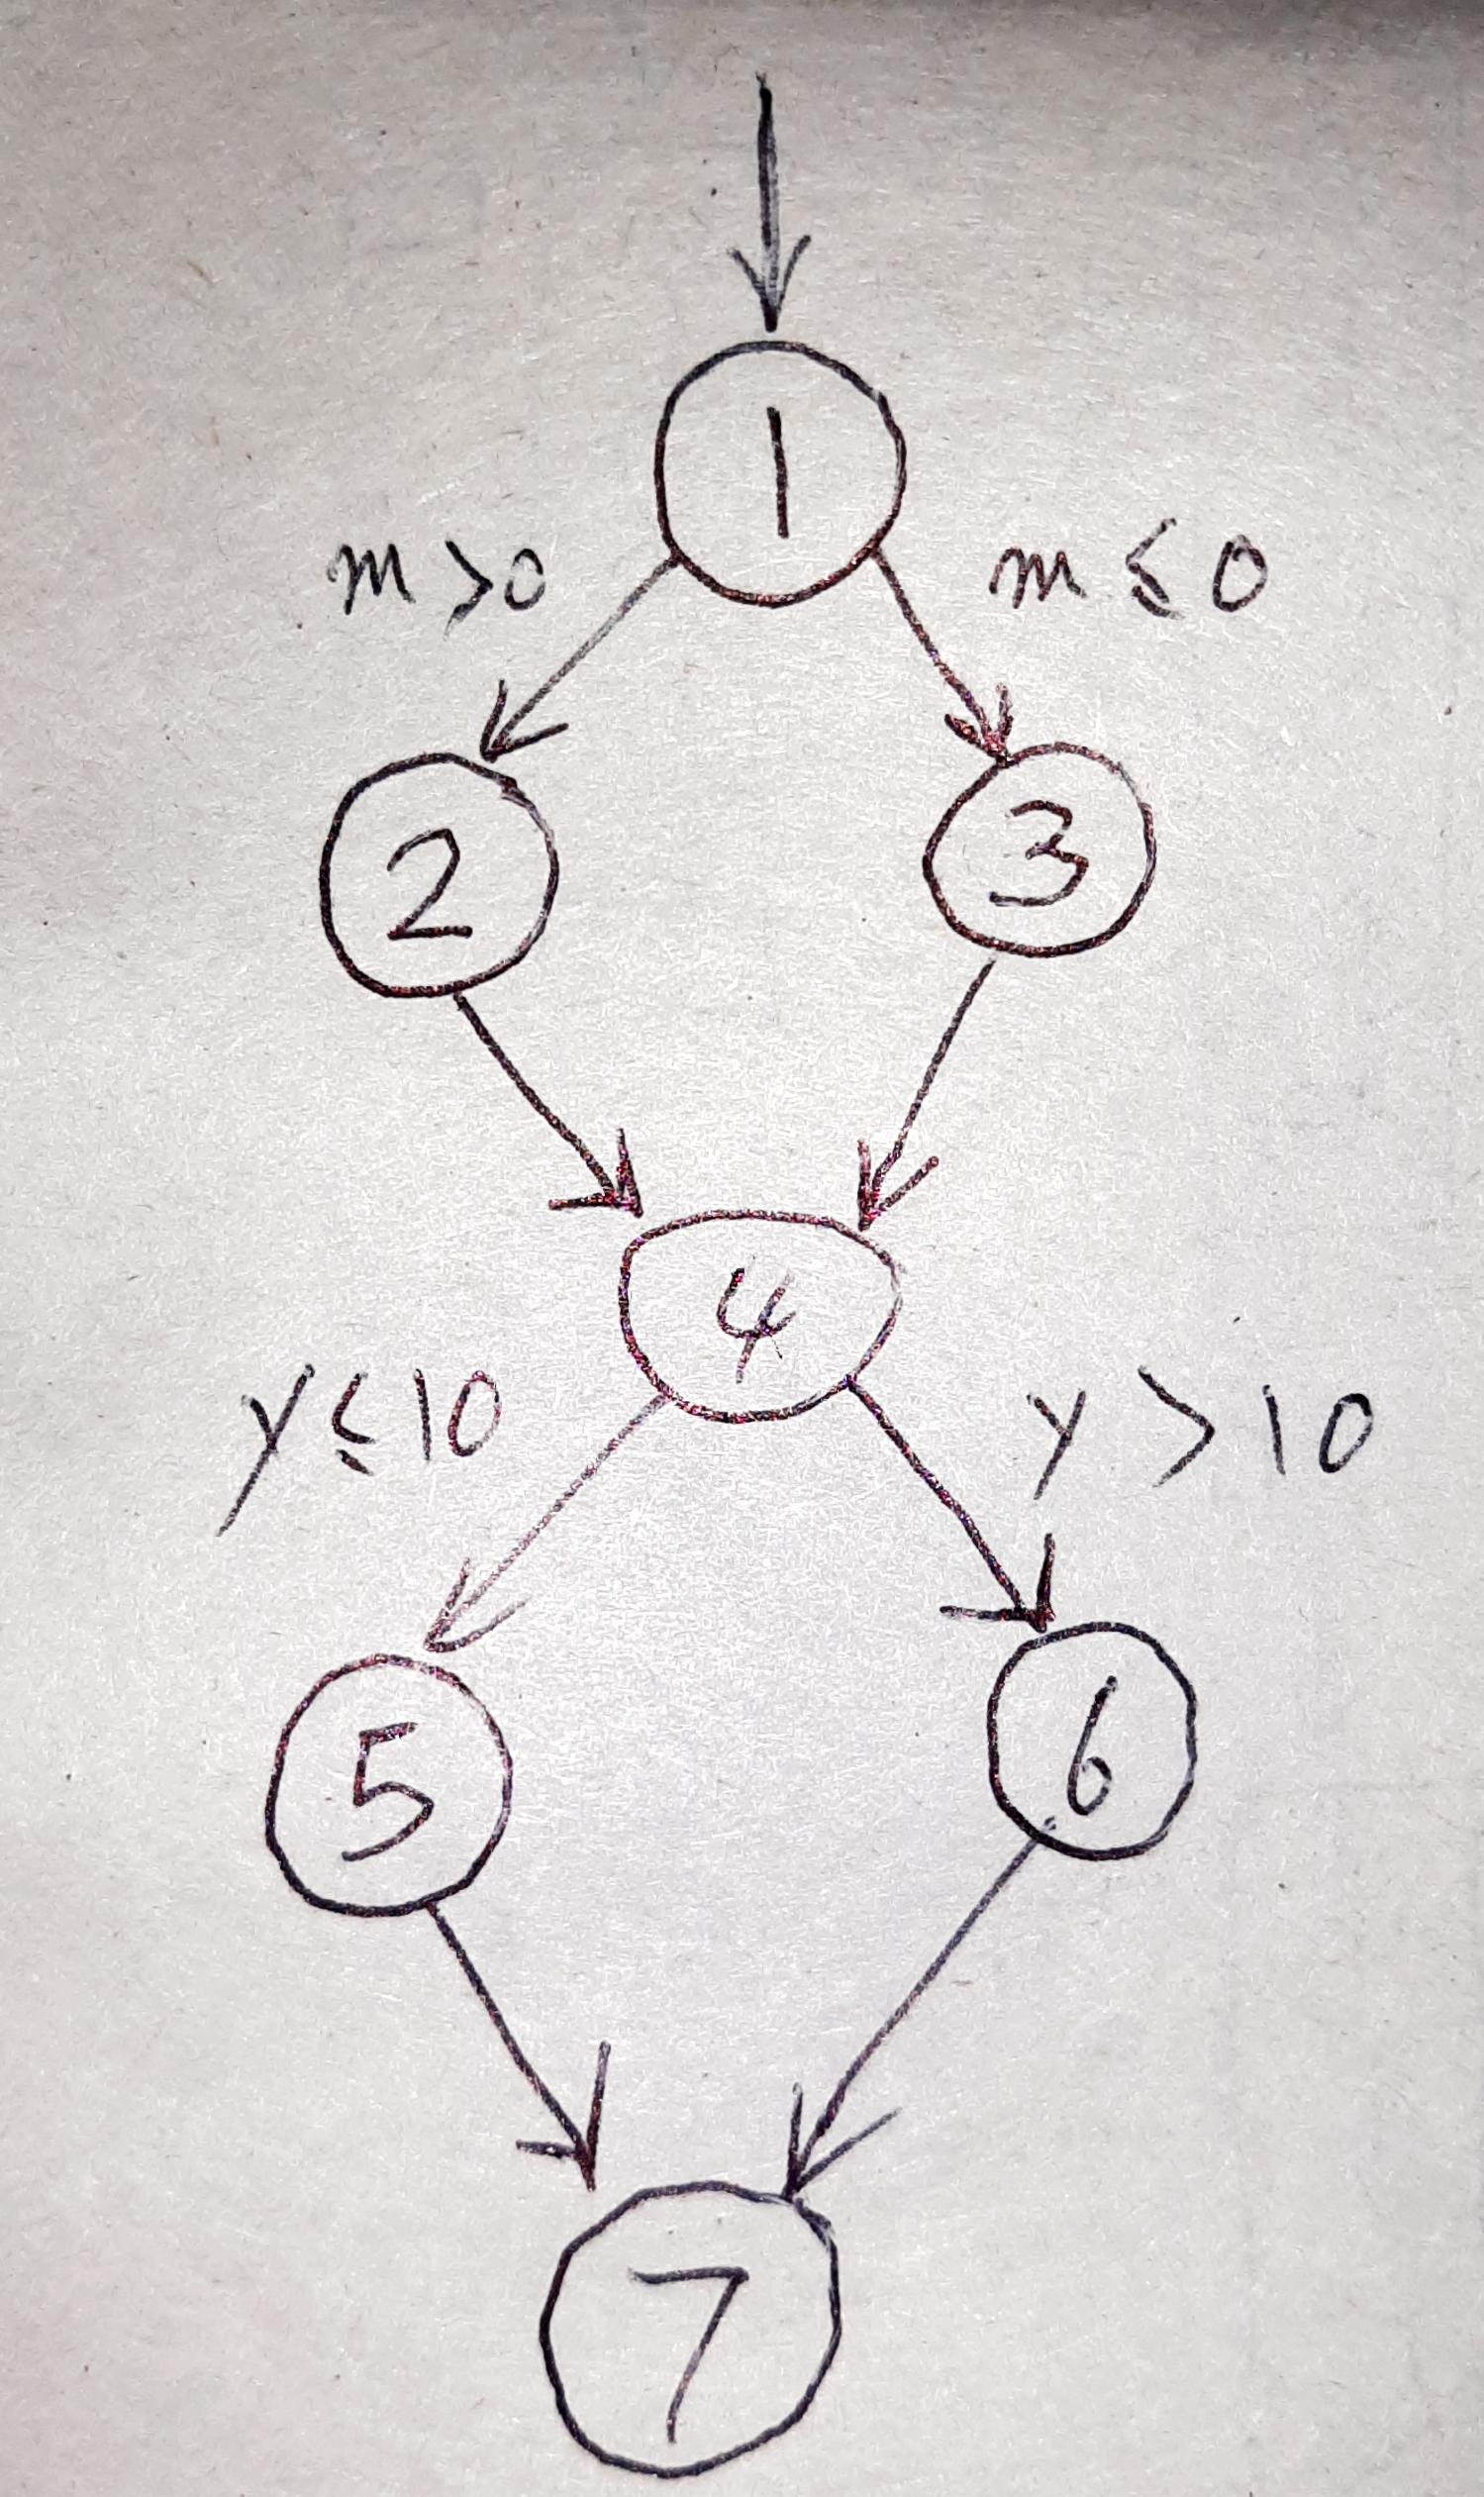
\includegraphics[width=0.25\textwidth]{figures/swt2.jpg}
    \caption
	{}
    \label{fig:fig1}
\end{figure}
\subsection{\lr{b}}
1 و 2 و 3
\subsection{\lr{c}}
2 و 3 و 7
\subsection{\lr{d}}
خیر-از آنجایی که در نودهای 2 و 3 متغیر \lr{w} \lr{def} شده است و نتیجتا از نود 1 تا نود 7 مسیر \lr{def-clear} نداریم. پس \lr{du-path} نیز نداریم.
\subsection{\lr{e}}
\begin{latin}
$
w:\:\:\:\:\:\:\:\:(2, 4, 5, 7), (3, 4, 5, 7), (2, 4, 6, 7), (3, 4, 6, 7)\\
x:\:\:\:\:\:\:\:\:(5, 7), (6, 7)
$
\end{latin}

\section{سوال‌های 3 و 4 صفحات 218 و 219}


\subsection{سوال 3}

\subsubsection{\lr{a}}
\begin{figure}[H]
    \centering
    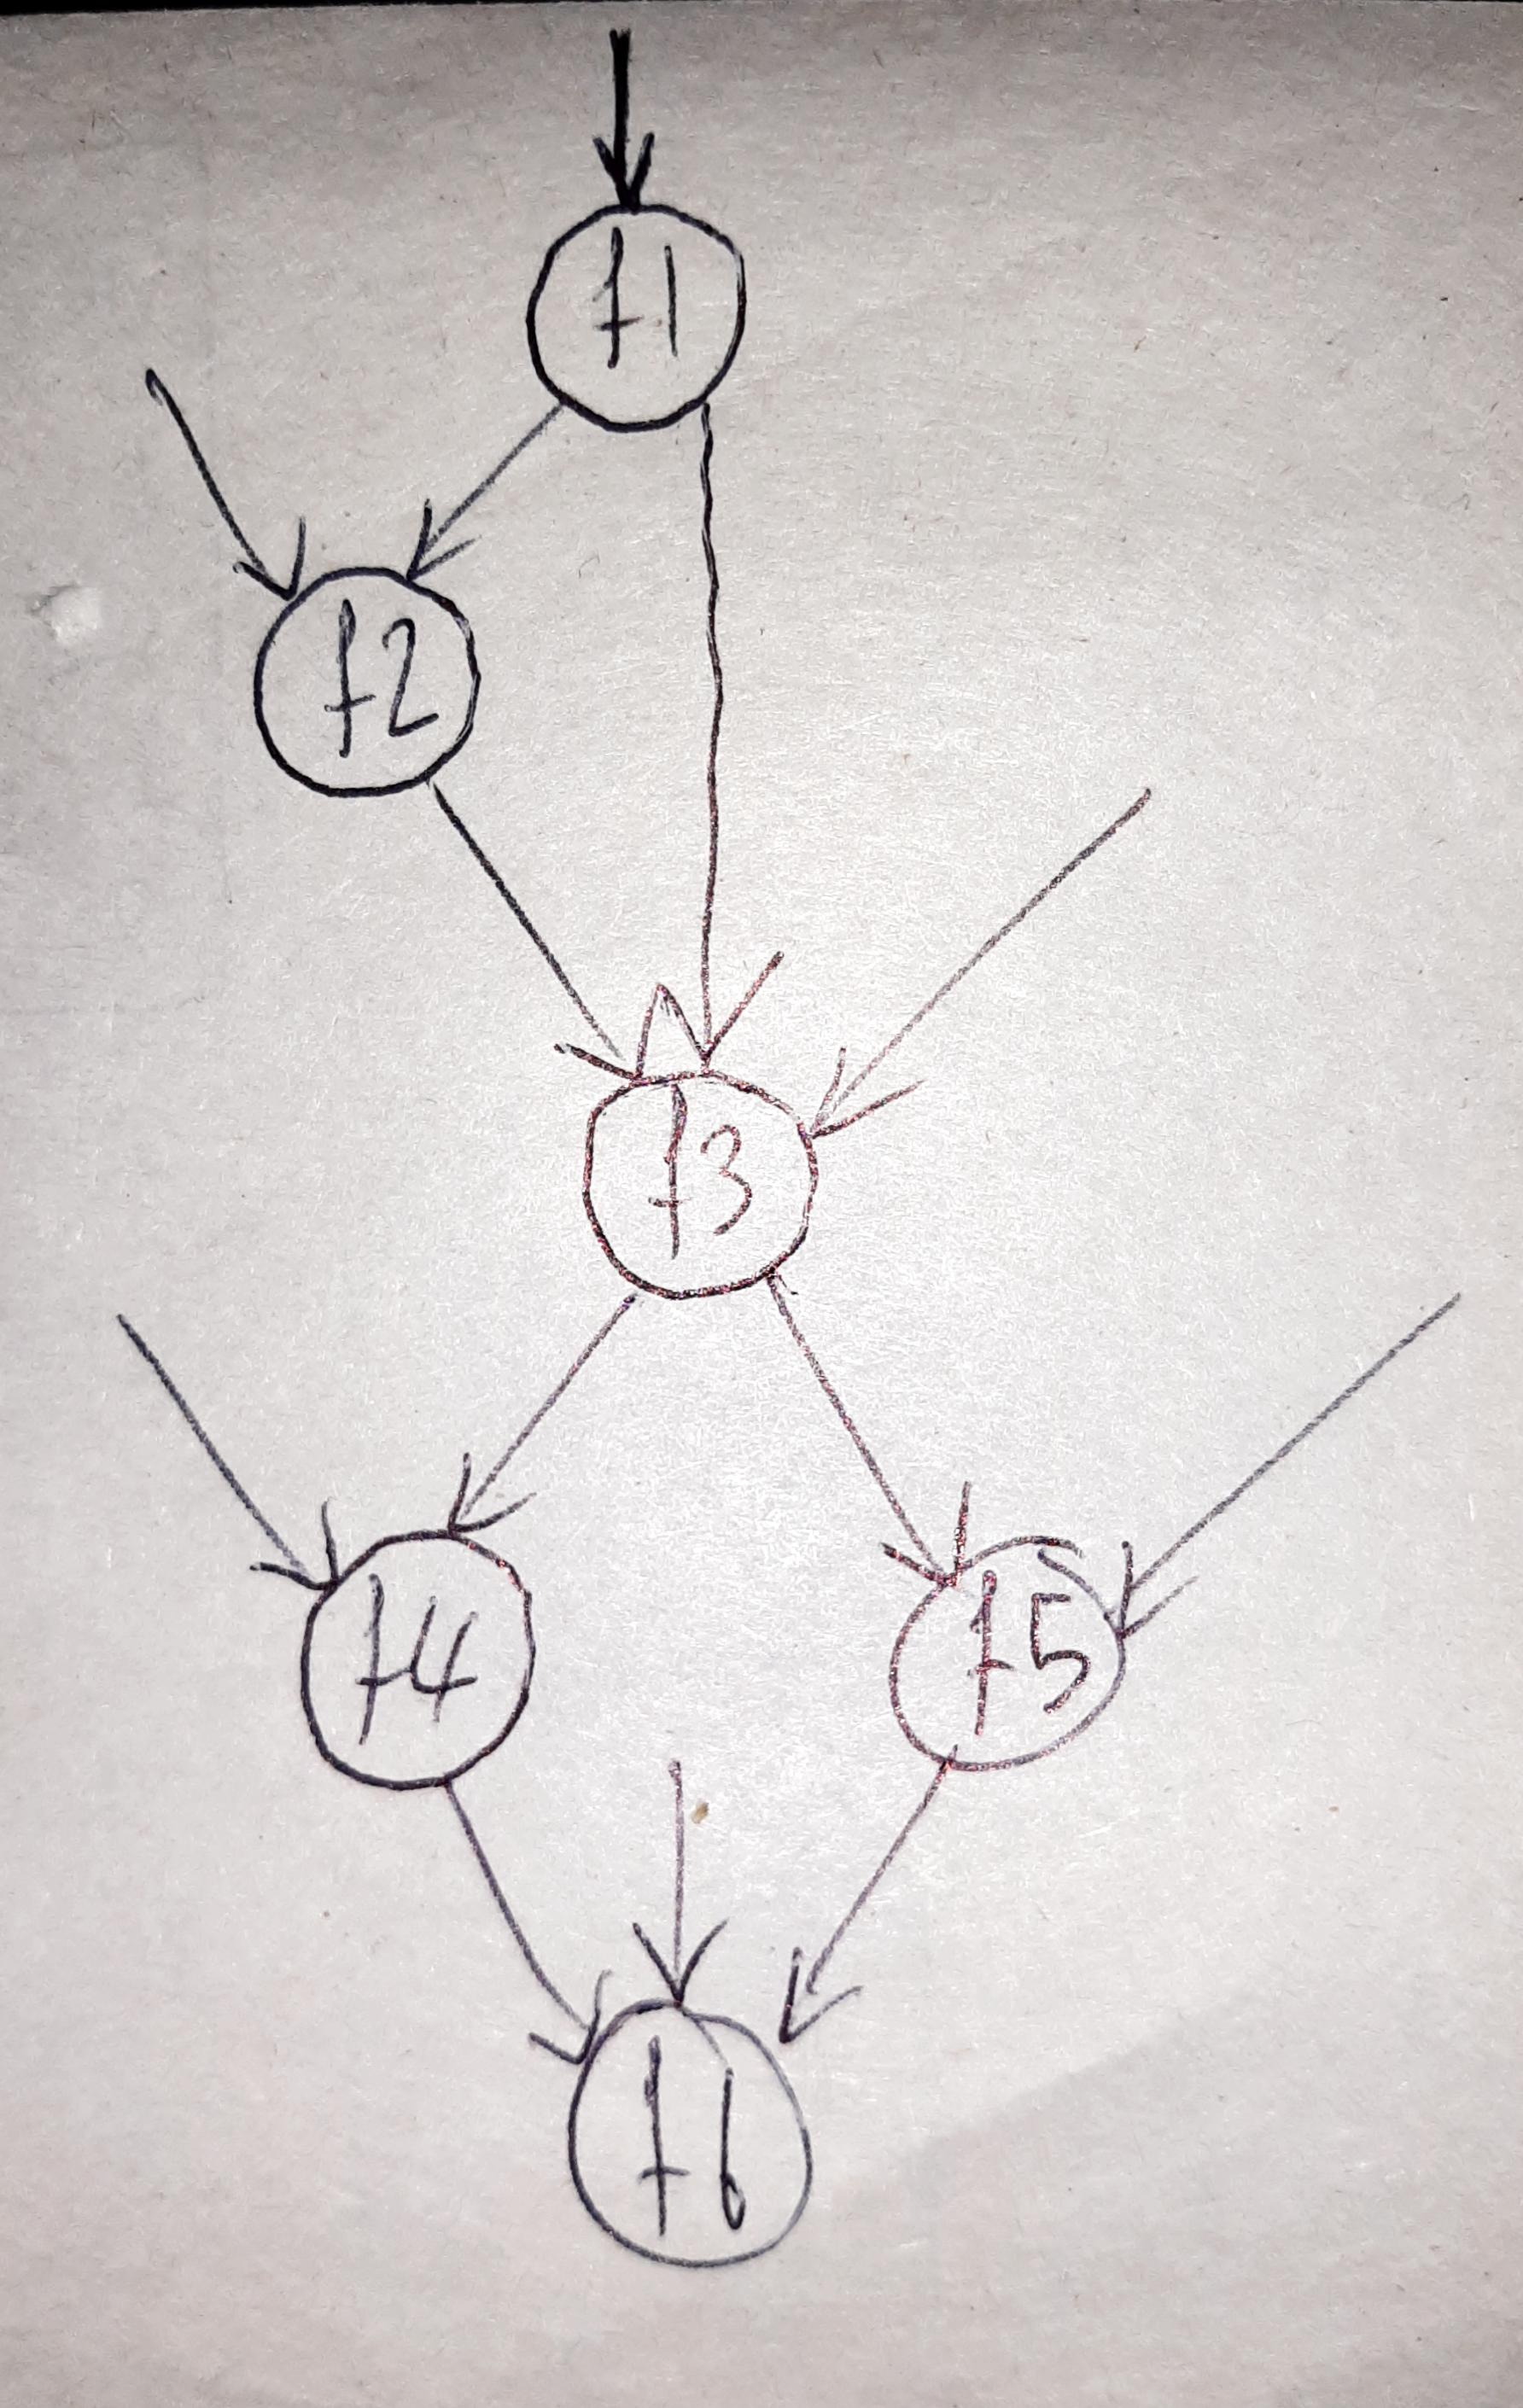
\includegraphics[width=0.25\textwidth]{figures/swt3.jpg}
    \caption
	{}
    \label{fig:fig1}
\end{figure}
\subsubsection{\lr{b}}
\begin{latin}
$
t1:\:\:\:\:\:\:\:\: [f1, f3, f5, f6]\\
t2:\:\:\:\:\:\:\:\: [f1, f3, f4, f6]\\
t3:\:\:\:\:\:\:\:\: [f1, f2]\\
t4:\:\:\:\:\:\:\:\: [f1, f3, f4, f6]\\
t5:\:\:\:\:\:\:\:\: [f1, f2, f3, f4, f6]\\
$
\end{latin}

\subsubsection{\lr{c}}
\begin{latin}
$
\left\{ t1, t5\right\}
$
\end{latin}

\subsubsection{\lr{d}}
\begin{latin}
$
\left\{ t1, t5\right\}
$
\end{latin}

\subsubsection{\lr{e}}
\begin{latin}
$
\left\{[f1, f3, f4, f6], [f1, f3, f5, f6], [f1, f2, f3, f4, f6], [f1, f2, f3, f5, f6]\right\}
$
\end{latin}
هیچ یک از مسیرهای تست $[f1, f2, f3, f5, f6]$ را پوشش نمی‌دهند.

\subsection{سوال 4}

\subsubsection{\lr{a}}
\begin{latin}
\begin{itemize}
\item Line 12: Calling \texttt{takeOut()} method in the \texttt{trash()} method.
\item Line 20: Calling \texttt{takeOut()} method in the \texttt{takeOut()} method.
\end{itemize}
\end{latin}
خط 12 و خط 13
\subsubsection{\lr{b}}
\begin{latin}
$
last-defs:\:\:\:\:\:\:\:\:  (x,1), (n,9), (n,11), (m,5), (m,7), (e,21), (e,23), (d,19), (a,15), (b,15)\\
first-uses:\:\:\:\:\:\:\:\:  (o,13), (a,19), (b,21), (b,23), (x,6), (m,9), (m,11), (n,12), (e,24), (d,21), (d,23)\\
$
\resizebox{.99\hsize}{!}
{$
all pairs:\:\:\:\:\:\:\:\:
(trash(), n, 9), (trash(), n, 9), (takeOut(), b, 21), (trash(), m, 5), (takeOut(), a, 19)
(trash(), n, 11), (takeOut(), b, 21), (takeOut(), b, 23), (trash(), m, 7), (takeOut(), a, 19),
(takeOut(), e, 21), (trash(), o, 13), (trash(), n, 11), (takeOut(), b, 23), (takeOut(), e, 23),
(trash(), o, 13)
$}
For the \texttt{trash()} method:
\begin{itemize}
\item Last-def: Line 7 (\texttt{m = 4})
\item First-use: Line 9 (\texttt{n = 3m})
\item Last-def: Line 11 (\texttt{n = 4m})
\item First-use: Line 12 (\texttt{takeOut(m, n)})\\
\end{itemize}
For the \texttt{takeOut()} method:
\begin{itemize}
\item Last-def: Line 19 (\texttt{d = 42a})
\item First-use: Line 21 (\texttt{e = 2b+d})
\item Last-def: Line 23 (\texttt{e = b+d})
\item First-use: Line 24 (\texttt{return e})
\end{itemize}
\end{latin}


\subsubsection{\lr{c}}
\begin{latin}
\begin{itemize}
\item Input: $x=10$
\item Explanation: The condition $x>0$ is true, so $m=4$. Then the nested condition $x>5$ is also true, so $n=3∗m=12$. The call to \texttt{takeOut(m, n)} will pass $m=4$ and $n=12$ as arguments. The expected output will depend on the implementation of the \texttt{takeOut()} method.
\end{itemize}
\end{latin}


\section{سوال اول صفحات 233 و 234}
\begin{latin}
\subsection{\lr{a}}
The variable "elements" in the \texttt{BoundedQueue2} class represents the elements present in the queue. Since we do not care about the specific objects, there are four useful values for this variable:

\begin{enumerate}
\item \texttt{null}: Represents an empty position in the queue.
\item \texttt{obj}: Represents a non-null object stored in the queue.
\item \texttt{obj1}: Represents a non-null object different from \texttt{obj} stored in the queue.
\item \texttt{obj2}: Represents another non-null object different from \texttt{obj} and \texttt{obj1} stored in the queue.
\end{enumerate}

\subsection{\lr{b}}
To determine the number of states, we need to consider all possible combinations of the representation variables \texttt{[elements, size, front, back]}. Let's analyze each variable:

\begin{itemize}
\item \texttt{elements}: There are 4 useful values for this variable (as discussed in part (a)).
\item \texttt{size}: The size can range from 0 to nn (the maximum capacity of the queue).
\item \texttt{front}: The front can range from 0 to $n−1$.
\item \texttt{back}: The back can range from 0 to $n−1$.
\end{itemize}

Considering these ranges, the total number of states is $(4×(n+1)×n×n)$, where nn is the maximum capacity of the queue.

\subsection{\lr{c}}
The reachable states are those that can be reached through valid method calls and operations on the \texttt{BoundedQueue2} object. To determine the number of reachable states, we need to identify the valid transitions between states based on the methods \texttt{enQueue()} and \texttt{deQueue()}.

\subsection{\lr{d}}
Since the exact maximum capacity $(n)$ of the queue is not specified, I cannot provide a specific drawing of the reachable states without this information.

\subsection{\lr{e}}
Adding edges for the \texttt{enQueue()} and \texttt{deQueue()} methods:

\begin{itemize}
\item \texttt{enQueue()}: This method adds an element to the back of the queue if it is not full. It updates the \texttt{elements}, \texttt{size}, and \texttt{back} variables accordingly.

\begin{enumerate}
\item If the queue is not full:
\begin{itemize}
\item Transition: \texttt{[elements, size, front, back]} →→ \texttt{[updated elements, updated size, front, updated back]}
\end{itemize}

\item If the queue is full (Exceptional Return):
\begin{itemize}
  \item Transition: \texttt{[elements, size, front, back]} $\rightarrow$ \texttt{[elements, size, front, back]}
\end{itemize}

\end{enumerate}

\item \texttt{deQueue()}: This method removes the element at the front of the queue if it is not empty. It updates the \texttt{elements}, \texttt{size}, and \texttt{front} variables accordingly.

\begin{enumerate}
\item If the queue is not empty:
\begin{itemize}
\item Transition: \texttt{[elements, size, front, back]} →→ \texttt{[updated elements, updated size, updated front, back]}
\end{itemize}

\item If the queue is empty (Exceptional Return):
\begin{itemize}
  \item Transition: \texttt{[elements, size, front, back]} $\rightarrow$ \texttt{[elements, size, front, back]}
\end{itemize}

\end{enumerate}

\end{itemize}

\subsection{\lr{f}}
To achieve Edge Coverage, we need to design a test set that covers all possible edges or transitions between states. Since the specific maximum capacity (n) of the queue is not provided, it's challenging to provide a complete test set without this information. However, here's an example of a small test set:

\begin{itemize}
\item Create an empty queue with a capacity of 3.
\item Call enQueue(obj1).
\item Call enQueue(obj2).
\item Call deQueue().
\item Call enQueue(obj3).
\end{itemize}

This test set covers the following edges:

\begin{itemize}
\item Initial state to state with one element: [[null, null], 0, 0, 0] -> [[obj1, null], 1, 0, 1]
\item State with one element to state with two elements: [[obj1, null], 1, 0, 1] -> [[obj1, obj2], 2, 0, 2]
\item State with two elements to state with one element: [[obj1, obj2], 2, 0, 2] -> [[null, obj2], 1, 1, 2]
\item State with one element to state with two elements again: [[null, obj2], 1, 1, 2] -> [[obj3, obj2], 2, 1, 0]
\end{itemize}

\end{latin}






%%%%%%%%%%%%%%%%%%%%%%%%%%%%%%%%%
%------------------------------------------------------------------------------------------
\end{document}